\documentclass{article}

\usepackage{fancyhdr}
\usepackage{extramarks}
\usepackage{amsmath}
\usepackage{amsthm}
\usepackage{amsfonts}
\usepackage{tikz}
\usepackage[plain]{algorithm}
\usepackage{algpseudocode}
\usepackage{enumitem}
\usepackage{pgfplots}
\usepackage{subcaption}

\usetikzlibrary{automata,positioning}

% Basic document settings
\topmargin=-0.45in
\evensidemargin=0in
\oddsidemargin=0in
\textwidth=6.5in
\textheight=9.0in
\headsep=0.25in

\linespread{1.1}

\pagestyle{fancy}
\lhead{\hmwkAuthorName}
\chead{\hmwkClass\ (\hmwkClassInstructor\ \hmwkClassTime): \hmwkTitle}
\rhead{\firstxmark}
\lfoot{\lastxmark}
\cfoot{\thepage}

\renewcommand\headrulewidth{0.4pt}
\renewcommand\footrulewidth{0.4pt}

\setlength\parindent{0pt}

% Pgfplots settings
\pgfplotsset{
    standard/.style={
        axis line style = thick,
        trig format=rad,
        enlargelimits,
        axis x line=middle,
        axis y line=middle,
        enlarge x limits=0.15,
        enlarge y limits=0.15,
        every axis x label/.style={at={(current axis.right of origin)}, anchor=north west},
        every axis y label/.style={at={(current axis.above origin)},anchor=south east},
        % grid=both,
        ticklabel style={font=\large, fill=white}
    }
}

% Create problem sections
\newcommand{\enterProblemHeader}[1]{
    \nobreak\extramarks{}{Problem \arabic{#1} continued on next page\ldots}\nobreak{}
    \nobreak\extramarks{Problem \arabic{#1}}{Problem \arabic{#1} continued on next page\ldots}\nobreak{}
}

\newcommand{\exitProblemHeader}[1]{
    \nobreak\extramarks{Problem \arabic{#1}}{Problem \arabic{#1} continued on next page\ldots}\nobreak{}
    \stepcounter{#1}
    \nobreak\extramarks{Problem \arabic{#1}}{}\nobreak{}
}

\setcounter{secnumdepth}{0}
\newcounter{partCounter}
\newcounter{homeworkProblemCounter}
\setcounter{homeworkProblemCounter}{1}
\nobreak\extramarks{Problem \arabic{homeworkProblemCounter}}{}\nobreak{}

% Homework problem environment
\newenvironment{homeworkProblem}[1][-1]{
    \ifnum#1>0
        \setcounter{homeworkProblemCounter}{#1}
    \fi
    \section{Problem \arabic{homeworkProblemCounter}}
    \setcounter{partCounter}{1}
    \enterProblemHeader{homeworkProblemCounter}
}{
    \exitProblemHeader{homeworkProblemCounter}
}

% Homework details
\newcommand{\hmwkTitle}{Problem Set\ \#4}
\newcommand{\hmwkDueDate}{November 12, 2024}
\newcommand{\hmwkDueTime}{1:00pm}
\newcommand{\hmwkClass}{Macroeconomics}
\newcommand{\hmwkClassTime}{Section 104}
\newcommand{\hmwkClassInstructor}{Prof. Barnichon}
\newcommand{\hmwkAuthorName}{\textbf{Zachary Brandt}}

% Title page
\title{
    \vspace{2in}
    \textmd{\textbf{\hmwkClass:\ \hmwkTitle}}\\
    \normalsize\vspace{0.1in}\small{Due\ on\ \hmwkDueDate\ at \hmwkDueTime}\\
    \vspace{0.1in}\large{\textit{\hmwkClassInstructor\ \hmwkClassTime}}
    \vspace{3in}
}

\author{\hmwkAuthorName}
\date{}

% Various helper commands 

\renewcommand{\part}[1]{\textbf{\large Part \Alph{partCounter}}\stepcounter{partCounter}\\}

% Useful for algorithms
\newcommand{\alg}[1]{\textsc{\bfseries \footnotesize #1}}

% For derivatives
\newcommand{\deriv}[1]{\frac{\mathrm{d}}{\mathrm{d}x} (#1)}

% For partial derivatives
\newcommand{\pderiv}[2]{\frac{\partial}{\partial #1} (#2)}

% Integral dx
\newcommand{\dx}{\mathrm{d}x}

% Alias for the Solution section header
\newcommand{\solution}{\textbf{\large Solution}}

% Probability commands: Expectation, Variance, Covariance, Bias
\newcommand{\E}{\mathrm{E}}
\newcommand{\Var}{\mathrm{Var}}
\newcommand{\Cov}{\mathrm{Cov}}
\newcommand{\Bias}{\mathrm{Bias}}

\begin{document}

\maketitle

\pagebreak

\begin{homeworkProblem}[1]
    Consider the model of the medieval economy discussed in class: 
    
    \begin{enumerate}[topsep=15pt]
        \item[] \:\:\: $\log M_t + \log V = \log P_t + \log Y_t$
        \item[] \:\:\: $\log P_{t+1} - \log P_t = \theta (\log Y_t - \log Y^*)$
    \end{enumerate}
    
    A) Suppose $V=1$ and $Y^* = 1$. Calculate the steady state of this economy
    when $\log M_t = 1$.
    \\ \\
    B) Suppose that time is measured in years and the economy is in the steady
    calculate in part A) at time $t=-1$. Suppose that at time $t=0$ Vikings bring
    back a boatload of gold coins that raises the money supply to $\log M_0=3$.
    Suppose that the money supply remains constant at this level for the next
    20 years. Suppose that $\theta = 0.25$. Trace out the dynamics of the
    logarithm of the price level and the logarithm of output over these 20 years
    using the two equations from part A). Plot the resulting ''time series" for
    logarithm of output, the logarithm of the price level, and the logarithm
    of the money supply from $t=-1$ to $t=20$ (i.e. plot each variable as a 
    function of time).
    \\ \\
    C) Now suppose that $\theta = 0.5$. Trace out the dynamics in this case. 
    Again plot the results as in the previous part. 
    \\ \\
    D) Comment on the transiton dynamics and the difference between the two
    cases. Relate to the concept of the half-life (one paragraph). 
    
    \pagebreak
    \part
    
    Suppose $V=1$ and $Y^* = 1$. Calculate the steady state of this economy
    when $\log M_t = 1$.
    \\ \\
    \solution
    
    In the long run the economy will reach a steady state where the variables
    do not change across periods. In this case $P_{t+1} = P_t = P$, and we 
    can subtsitute in our values for $V$, $Y^*$, and $\log M_t$ into the
    given equations.
    \[
        \begin{split}
            \log P_{t+1} - \log P_t &= \theta (\log Y_t - \log Y^*)
            \\
            0 &= \theta(\log Y - \log(1))
            \\
            0 &= \log Y
            \\
            Y &= 1
        \end{split}
    \]
    \[
        \begin{split}
            \log M_t + \log V &= \log P_t + \log Y_t 
            \\
            1 + \log(1) &= \log P + \log Y 
            \\
            1 &= \log P + \log Y
            \\
            \log P &= 1
        \end{split}
    \]

    From the above we can see that the steady state value of $Y$ is 1, the
    same value as the desired level of output $Y^*$. The log of the price
    level is also 1, which is the same value as the log of the money
    supply. This suggests that there is a long-run monetary neutrality,
    in that prices and money supply change proportionally, but leave output
    unaffected.

    \pagebreak
    \part

    Suppose that time is measured in years and the economy is in the steady
    calculate in part A) at time $t=-1$. Suppose that at time $t=0$ Vikings bring
    back a boatload of gold coins that raises the money supply to $\log M_0=3$.
    Suppose that the money supply remains constant at this level for the next
    20 years. Suppose that $\theta = 0.25$. Trace out the dynamics of the
    logarithm of the price level and the logarithm of output over these 20 years
    using the two equations from part A). Plot the resulting ''time series" for
    logarithm of output, the logarithm of the price level, and the logarithm
    of the money supply from $t=-1$ to $t=20$ (i.e. plot each variable as a 
    function of time).
    \\ \\
    \solution 
    
    \begin{figure}[h]
        \centering
        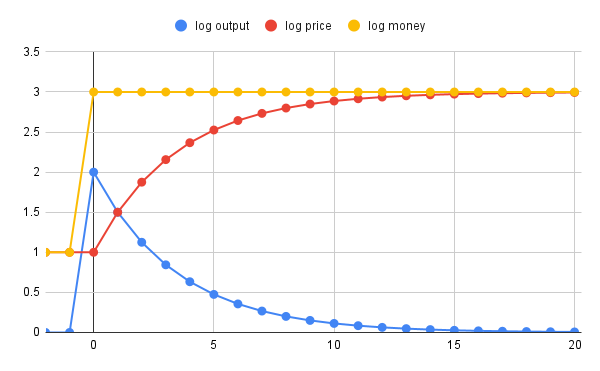
\includegraphics[width=1\textwidth]{partb.png}
                % \caption{This is an image caption.}
        \label{fig:example}
    \end{figure}
    
    \pagebreak
    \part

    Now suppose that $\theta = 0.5$. Trace out the dynamics in this case. 
    Again plot the results as in the previous part. 
    \\ \\
    \solution

    \begin{figure}[h]
        \centering
        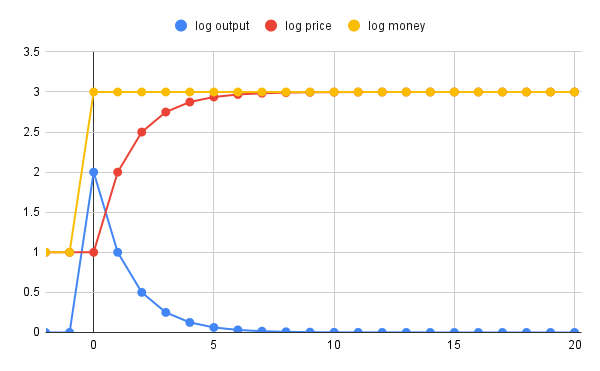
\includegraphics[width=1\textwidth]{partc.png}
        % \caption{This is an image caption.}
        \label{fig:example}
    \end{figure}

    \pagebreak
    \part

    Comment on the transiton dynamics and the difference between the two
    cases. Relate to the concept of the half-life (one paragraph). 
    \\ \\
    \solution

    Steady state logarithms of output and price are reached quicker in 
    the second case where the speed of the price adjustment, $\theta$,
    is equal to 0.5, whereas in the first case it is 0.25. The half-life
    is the time required for, in this case, the logarithms of output and
    price to reduce to half their value. In the second case, the half-life
    is then naturally shorter. This makes sense considering that, if prices
    take less time to adjust, suppliers will adjust prices quicker to
    catch up with inflated demand, thereby reducing output quicker as well. 
     

\end{homeworkProblem}

\pagebreak

\begin{homeworkProblem}[2]
    Indicate whether you think the following statements are true, false or 
    uncertain. Support your answer by giving all necessary reasoning and 
    calculations:
    \\ \\
    A) The discovery of large gold and silver mines in the Americas in the
    16\textsuperscript{th} century greatly increased the purchasing power
    of people in Europe.
    \\ \\
    \textbf{False}. The influx of gold and silver into a Europe where these 
    metals served as money did not broadly increase the purchasing power of 
    people. Purchasing power is the amount of goods and services one can buy
    with money. If only the money supply increases, all other things being 
    equal, this will simply cause an increase in prices, as producers adjust 
    prices to excess demand stimulated by an increase in the money supply.
    \\ \\
    
    B) According to the quantity theory of money, ``inflation is always
    and everywhere a monetary phenomenon.''
    \\ \\
    \textbf{True}. According to the quantity theory of money, the price
    level is directly proportional to the money supply, and that there is a 
    causality between changes in the money supply and changes in the price 
    level. The above statement corresponds with this idea, since it claims 
    that inflation (rising of prices), results from an increase in the money 
    supply. 
    
\end{homeworkProblem}

\pagebreak
\end{document}
